\section{Technische Grundlagen} - Technologische Grundlagen - Grundlagen /
\subsection{MQTT}
\acf{mqtt} wurde ursprünglich von Doktor Andy Stanford-Clark und Arlen Nipper im Jahr 1999 entworfen um Gas- und Ölpiplines zu überwachen. Diese lagen oftmals an entlegenen Orten, wie zum Beispiel auf Übersee, und konnten nicht mit Radiowellen oder einem Kabel zum Festland erreicht werden. Zu dieser Zeit war die einzige Option um Sensordaten auf einen Server zu übertragen eine auf Datendurchsatz abgerechnete Satellitenkommunikation. Bei mehreren tausend Sensoren wurde somit ein Protokoll benötigt, das die Daten zuverlässig mit minimaler Bandbreite an die Server auf dem Festland übermitteln kann.
\ac{mqtt} wurde im Jahr 2013 von der \ac{oasis} als Open Source standatisiert und wird heutzutage von vielen gro{\ss}en \ac{iot} Platformen unterstützt.\cite{WhatMQTTDefinition}\\
Es gibt derzeit zwei Versionen der MQTT Spezifikation: \verb|3.1.1| und \verb|5|. Alle Referenzen, falls nicht explizit gekennzeichnet, beziehen sich auf die aktuelle Version \verb|5| des Protokolls.\\
\ac{mqtt} ist ein Layer 7 \textit{Publish and Subscribe} Protkoll, das auf \acs{tcp} / \acs{ip} aufsetzt. Anders als das Request / Response Paradigma bei \acs{http} ist \ac{mqtt} Event gesteuert und erlaubt Nachrichten direkt an einen bestimmten Client zu schicken. Somit muss nicht periodisch nach neuen Nachrichten gefragt werden. Zusammen mit einem fixen Paket-Header von nur zwei Byte sorgen diese Eigeschaften für einen minimalen Datendurchsatz.\cite{WhatMQTTDefinition}

\subsubsection{Publish and Subscribe}
\ac{mqtt} nutzt das \textit{Publish and Subscribe} Kommunikationsschema, das eine Struktur bietet um Nachrichten zwischen Herausgeber und Abonnent auszutauschen. In diesem Schema gibt es zwei unterschiedliche Systeme:
\begin{itemize}
    \item Clients
    \item Broker
\end{itemize}
Clients sind alle Teilnehmer dieses Systems, die Nachricht empfangen oder veröffentlichen wollen. Diese setzten auf einen Broker als Mittelsmann um die Nachrichten erfolgreich zu vermitteln.\cite{teamGettingStartedMQTT} Jede Nachricht wird durch den Herausgeber in bestimmte Klassen kategorisiert. Der Herausgeber wei{\ss}t nicht ob, oder wer, an dieser Nachricht interessiert ist und schickt die klassifizierte Nachricht an den Broker. Clients, die an bestimmten Nachrichten interessiert sind, müssen bei dem Broker ein Abonnement erstellen und dabei die gewünschte Kategorie angeben. Somit kann der Broker eingehende kategorisierte Nachrichten an die entsprechenden Clients weiterleiten. Der Broker kann Nachrichten zudem auch aufbewahren, sodass Clients, die zu einem späteren Zeitpunkt auf ein Thema abonnieren, ebenfalls die vergangenen Nachrichten erhalten. Durch dieses System entsteht eine Entkopplung der einzelnen Clients auf mehreren Ebenen.\cite{EverythingYouNeed}
\begin{itemize}
    \item \textbf{Räumliche Entkopplung:} Herausgeber und Abonnent der Nachricht müssen sich nicht kennen.
    \item \textbf{Zeitliche Entkopplung:} Herausgeber und Abonnent müssen nicht zur selben Zeit aktiv sein.
    \item \textbf{Synchronisierungs Entkopplung:} Herausgeber und Abonnent müssen ihre Operationen beim publizieren und konsumieren nicht unterbrechen. TODO warum?:
\end{itemize}
\cite{teamPublishSubscribeMQTT}
In verteilten System, wo einzelne Komponenten oftmals sehr unterschiedlich sind, spielt ein solches Konzept eine gro{\ss}e Rolle, da es eine einheitliche Abstraktion der Kommunikationsebene bietet.\cite{domingusDistributedSystemsIntroduction2020}
% TODO mehr zu distributed systems
% TODO bild publisher - subscriber topic
% TODO bild von sensoren / broker / downstream clients
\begin{figure}
    \centering
    %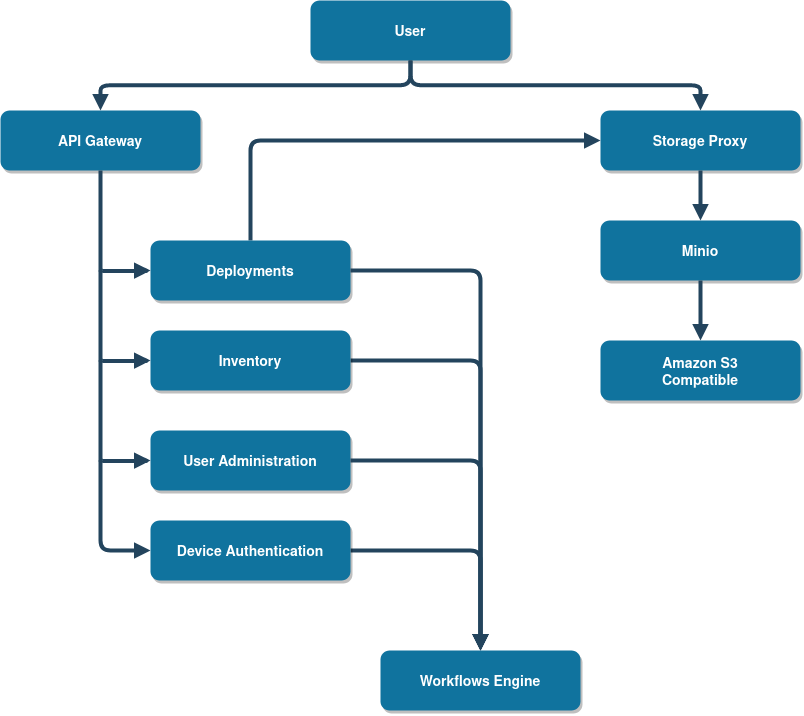
\includegraphics[scale=0.5]{images/integration-app.png}
    \caption{Publish and Subscribe Architektur basirend auf Themen}
    \label{fig:publish-subscribe}
\end{figure}
Im Kontext \ac{mqtt} werden Nachrichten in eine hieraschich aufgebaute Themenstruktur klassifiziert. Themen werden mit einem Schrägstrich (\verb|/|) getrennt und sehen zum Beispiel wie folgt aus: \verb|sensors/temperature/celcius|. Abbildung \ref{fig:publish-subscribe} zeigt einen Client, der auf das Thema \verb|bla| Nachrichten veröffentlicht. Diese wird an zwei weitere Clients durch den Broker weitergeleitet, da diese das Thema \verb|bla| abonniert haben. Themen müssen auf einem Broker nicht explizit angelegt werden. Sobald ein Client auf einem Thema publiziert oder es abonniert, wird dieses automatisch angelegt.\cite{WhatMQTTDefinition}\\
Beim abonnieren eines Themas kann entweder ein spezifisches Thema oder eine Kombination aus Thema und Wildcard verwendet werden. Bei einer Wildcard werden zwischen den folgenden zwei unterschieden:\cite{mqtt5Specification}
\begin{itemize}
    \item Multi-level '\verb|#|': Schlie{\ss}t das Vorgänger- und alle nachfolgenden Themen mit ein.
    \item Single-level '\verb|+|': Schlie{\ss}t alle Themen auf einer einzigen Ebene mit ein.
\end{itemize}
Bei der folgenden Themenstruktur
\begin{itemize}
    \item \verb|sensors|
    \item \verb|sensors/temperature|
    \item \verb|sensors/temperature/celcius|
    \item \verb|sensors/temperature/kelvin|
    \item \verb|sensors/fuel|
    \item \verb|sensors/fuel/tank1|
    \item \verb|sensors/fuel/tank2|
\end{itemize}
schlie{\ss}t ein Abonnement auf \verb|sensors/#| alle Themen mit ein. Bei einem Abonnement auf \verb|sensors/+| sind hingegen nur diese Themen mit eingeschlossen:
\begin{itemize}
    \item \verb|sensors/temperature|
    \item \verb|sensors/fuel|
\end{itemize}

\subsubsection{Quality of Service}
Je zuverlässiger eine Nachricht übermittelt werden soll, desto mehr Datendurchsatz verursacht diese Nachricht im gesamten System. Wenn ein Client wissen will, ob seine Nachricht im Broker eingetroffen ist, muss der Broker dem Client eine entsprechende Rückmeldung geben. Andernfalls kann der Client seine Nachricht an den Broker schicken ohne eine Rückmeldung zu erwarten. Dies ist vergleichsweise im \ac{http} nicht möglicht. Dort muss auf jede Nachricht geantwortet werden.\\
Bei \ac{mqtt} wird die Zuverlässigkeit der Übermittlung einer Nachricht mit einem \textit{\acf{qos}} Level festgelegt. Eine Nachricht publizierte Nachricht muss einen der drei \ac{qos} Level haben:
\begin{itemize}
    \item \ac{qos} 1: Maximal eine Zustellung der Nachricht.
    \item \ac{qos} 2: Mindestens eine Zustellung der Nachricht.
    \item \ac{qos} 3: Genau eine Zustellung der Nachricht.
\end{itemize}
Bei \ac{qos} Level 2 und 3 werden Handshakes zur Verifizierung der Paketübermittelung eingesetzt.\cite{mqtt5Specification}

\subsubsection{Paket Struktur}
\ac{mqtt} hat die Absicht ein leichtgewichtiges Protokoll zu sein. Tabelle \ref{table:mqtt-packet-structure} zeigt den Aufbau eines jeden \ac{mqtt} Paketes. Die fixe Kopfzeile ist zwei Byte gro{\ss} und muss in jedem Paket vorhanden sein. Basierend auf der Art des Paketes, das in der fixen Kopfzeile angegeben wird, sind zusätzlich eine variable Kopfzeile und weitere Daten möglich.\cite{mqtt5Specification}
\begin{table}[h!]
\centering
\renewcommand{\arraystretch}{1.5}
\begin{tabular}{|c|}
    \hline
    Fixe Kopfzeile, muss in jedem \ac{mqtt} Paket vorhanden sein \\
    \hline
    Variable Kopfzeile, optional \\
    \hline
    Daten des Pakets, optional \\
    \hline
\end{tabular}
\caption{Struktur eines \ac{mqtt} Paketes}
\label{table:mqtt-packet-structure}
\end{table}
Tabelle \ref{table:fixed-header} zeigt den detaillierten Aufbau der fixen Kopfzeile. Im ersten Byte werden Bit sieben bis vier für die spezifische Art des Paketes verwendet. Tabelle \ref{table:mqtt-packet-types} enhält eine Liste mit allen möglichen Pakettypen und deren Wert. Byte zwei gibt die restliche Paketlänge encodiert als \textit{Variable Byte Integer} an. Die Restliche Paketlänge setzt sich aus ... zusammen. Ein \textit{Variable Byte Integer} ist ... . Die maximale Paketgrö{\ss}e beträgt ... .\cite{mqtt5Specification}
% TODO was ist ein variable byte integer
% TODO wie setzt sich die restliche paketlänge zusammen
\begin{table}[h!]
\centering
\renewcommand{\arraystretch}{1.5}
\begin{tabularx}{\textwidth}{|l| *{8}{Y|}}
    \hline
    Bit & 7 & 6 & 5 & 4 & 3 & 2 & 1 & 0 \\
    \hline
    \hline
    Byte 1 & \multicolumn{4}{c|}{\ac{mqtt} Paketart} & \multicolumn{4}{c|}{Paketart spezifische Kennzeichnung} \\
    \hline
    Byte 2 & \multicolumn{8}{c|}{Restliche Paketlänge} \\
    \hline
\end{tabularx}
\caption{Aufbau der fixen \ac{mqtt} Kopfzeile}
\label{table:fixed-header}
\end{table}

\begin{table}[h!]
\centering
\renewcommand{\arraystretch}{1.5}
\begin{tabular}{|l|c|}
    \hline
    \textbf{Name} & \textbf{Wert} \\
    \hline
    \hline
    Reserved & 0 \\
    \hline
    CONNECT & 1 \\
    \hline
    CONNACK & 2 \\
    \hline
    PUBLISH & 3 \\
    \hline
    PUBACK & 4 \\
    \hline
    PUBREC & 5 \\
    \hline
    PUBREL & 6 \\
    \hline
    PUBCOMP & 7 \\
    \hline
    SUBSCRIBE & 8 \\
    \hline
    SUBACK & 9 \\
    \hline
    UNSUBSCRIBE & 10 \\
    \hline
    UNSUBACK & 11 \\
    \hline
    PINGREQ & 12 \\
    \hline
    PINGRESP & 13 \\
    \hline
    DISCONNECT & 14 \\
    \hline
    AUTH & 15 \\
    \hline
\end{tabular}
\caption{Verfügbare \ac{mqtt} Paketarten und deren Wert}
\label{table:mqtt-packet-types}
\end{table}

\subsubsection{MQTT CONNECT}
Nachdem eine Netzwerkverbindung zwischen einen Client und einem Broker aufgebaut wurde, muss das erste Paket eines Clients ein \verb|CONNECT| Paket sein. Tabelle \ref{table:mqtt-connect-packet-variable-header} zeigt den Aufbau und Inhalt einer Beispielhaften variablen Kopfzeile eines \verb|CONNECT| Paketes. Die ersten sechs Byte geben den Namen es Protokolls als UTF-8 encodierten String an. Dieser wird sich in zukünftigen Versionen nicht ändern und dient als Identifikationsmerkmal des \ac{mqtt} Protokolls für Server, die mehrere Protokolle implementiert haben.
\begin{table}[h!]
\centering
\renewcommand{\arraystretch}{1.5}
\begin{tabularx}{\textwidth}{|l|l|c| *{8}{Y|}}
    \hline
    & \textbf{Beschreibung} & \textbf{Wert} &
      \textbf{7} & \textbf{6} & \textbf{5} &
      \textbf{4} & \textbf{3} & \textbf{2} &
      \textbf{1} & \textbf{0} \\
    \hline
    \hline
    Byte 1 & Länge \acs{msb} & 0 & 0 & 0 & 0 & 0 & 0 & 0 & 0 & 0 \\
    \hline
    Byte 2 & Länge \acs{lsb} & 4 & 0 & 0 & 0 & 0 & 0 & 1 & 0 & 0 \\
    \hline
    Byte 3 & UTF-8 Char & 'M' & 0 & 1 & 0 & 0 & 1 & 1 & 0 & 1 \\
    \hline
    Byte 4 & UTF-8 Char & 'Q' & 0 & 1 & 0 & 1 & 0 & 0 & 0 & 1 \\
    \hline
    Byte 5 & UTF-8 Char & 'T' & 0 & 1 & 0 & 1 & 0 & 1 & 0 & 0 \\
    \hline
    Byte 6 & UTF-8 Char & 'T' & 0 & 1 & 0 & 1 & 0 & 1 & 0 & 0 \\
    \hline
    Byte 7 & Protokoll Version & 5 & 0 & 0 & 0 & 0 & 0 & 1 & 0 & 1 \\
    \hline
    Byte 8 &
        \makecell[l]{Benutzername Kennzeichnung \\ Passwort Kennzeichnung \\ 'Will' speichern \\ 'Will' \ac{qos} Level \\ 'Will' Kennzeichnung \\ Frischer Start \\ Reserviert} &
        \makecell{1 \\ 1 \\ 0 \\ 01 \\ 1 \\ 1 \\ 0} &
        1 & 1 & 0 & 0 & 1 & 1 & 1 & 0 \\
    \hline
    Byte 9 & Keep Alive \acs{msb} & 0 & 0 & 0 & 0 & 0 & 0 & 0 & 0 & 0 \\
    \hline
    Byte 10 & Keep Alive \acs{lsb} & 10 & 0 & 0 & 0 & 0 & 1 & 0 & 1 & 0 \\
    \hline
    Byte 11 & Länge der Eigenschaften & 0 & 0 & 0 & 0 & 0 & 0 & 0 & 0 & 0 \\
    \hline
\end{tabularx}
\caption{Verfügbare \ac{mqtt} Paketarten und deren Wert}
\label{table:mqtt-connect-packet-variable-header}
\end{table}

\subsubsection{Shared Subscriptions}


\newpage

\subsection{HiveMQ Broker}
\subsubsection{HiveMQ Cluster}
\subsection{Load Balancing}
was für load balancer gibt es ?
\subsection{Envoy}
vielleicht hier noch kein envoy ? ist dies grundlage oder teil der arbeit das wir uns für envoy entscheiden ?

If your work makes use of existing non-standard systems, tools, frameworks, librariesetc. describe these as well. However, just give a broad overview and delve just into those details that are crucial for the understanding of the following chapters. For standard sys-tems, tools, frameworks, and libraries please refer to its authoritative documentation. Youare not supposed to give an thorough introduction into, e.g., Java or ReactJS.

